%%%%%%%%%%%%%%%%%%%%%%%%%%%%%%%%%%%%%%%%%%%%%%%%%%%%%%%%%%%%%%%%%%%%%%%%%%%%%%%%%%%%%%%%%%%%%%%%
%
% CS484 Written Question Template
%
% Acknowledgements:
% The original code is written by Prof. James Tompkin (james_tompkin@brown.edu).
% The second version is revised by Prof. Min H. Kim (minhkim@kaist.ac.kr).
%
% This is a LaTeX document. LaTeX is a markup language for producing 
% documents. Your task is to fill out this document, then to compile 
% it into a PDF document. 
%
% 
% TO COMPILE:
% > pdflatex thisfile.tex
%
% If you do not have LaTeX and need a LaTeX distribution:
% - Personal laptops (all common OS): www.latex-project.org/get/
% - We recommend latex compiler miktex (https://miktex.org/) for windows,
%   macTex (http://www.tug.org/mactex/) for macOS users.
%   And TeXstudio(http://www.texstudio.org/) for latex editor.
%   You should install both compiler and editor for editing latex.
%   The another option is Overleaf (https://www.overleaf.com/) which is 
%   an online latex editor.
%
% If you need help with LaTeX, please come to office hours. 
% Or, there is plenty of help online:
% https://en.wikibooks.org/wiki/LaTeX
%
% Good luck!
% Min and the CS484 staff
%
%%%%%%%%%%%%%%%%%%%%%%%%%%%%%%%%%%%%%%%%%%%%%%%%%%%%%%%%%%%%%%%%%%%%%%%%%%%%%%%%%%%%%%%%%%%%%%%%
%
% How to include two graphics on the same line:
% 
% \includegraphics[width=0.49\linewidth]{yourgraphic1.png}
% \includegraphics[width=0.49\linewidth]{yourgraphic2.png}
%
% How to include equations:
%
% \begin{equation}
% y = mx+c
% \end{equation}
% 
%%%%%%%%%%%%%%%%%%%%%%%%%%%%%%%%%%%%%%%%%%%%%%%%%%%%%%%%%%%%%%%%%%%%%%%%%%%%%%%%%%%%%%%%%%%%%%%%

\documentclass[11pt]{article}

\usepackage[english]{babel}
\usepackage[utf8]{inputenc}
\usepackage[colorlinks = true,
            linkcolor = blue,
            urlcolor  = blue]{hyperref}
\usepackage[a4paper,margin=1.5in]{geometry}
\usepackage{stackengine,graphicx}
\usepackage{fancyhdr}
\setlength{\headheight}{15pt}
\usepackage{microtype}
\usepackage{times}
\usepackage{booktabs}
\usepackage{graphicx}

% From https://ctan.org/pkg/matlab-prettifier
\usepackage[numbered,framed]{matlab-prettifier}

\frenchspacing
\setlength{\parindent}{0cm} % Default is 15pt.
\setlength{\parskip}{0.3cm plus1mm minus1mm}

\pagestyle{fancy}
\fancyhf{}
\lhead{Project Writeup}
\rhead{CS 484}
\rfoot{\thepage}

\date{}

\title{\vspace{-1cm}Homework X Writeup}


\begin{document}
\maketitle
\vspace{-3cm}
\thispagestyle{fancy}

\section*{Instructions}
\begin{itemize}
  \item Describe any interesting decisions you made to write your algorithm.
  \item Show and discuss the results of your algorithm.
  \item Feel free to include code snippets, images, and equations.
  \item Use as many pages as you need, but err on the short side If you feel you only need to write a short amount to meet the brief, th
  
  \item \textbf{Please make this document anonymous.}
\end{itemize}
\newcommand\tab[1][1cm]{\hspace*{#1}}
\section*{Files}

{\large $1.$ get\_interest\_point.m \par}
\tab input : image, descriptor\_window\_image\_width. \\
\tab output : x, y, confidence, (scale), (orientation).

{\large $1.$ get\_descripotrs.m \par}
\tab input : image, x, y, descriptor\_window\_image\_width. \\
\tab output : features.

{\large $1.$ match\_features.m \par}
\tab input : features$1$, features$2$.\\
\tab output : matches, confidences.

\section*{Code}
{\large $1.$ my\_imfilter.m \par}
\begin{lstlisting}[style=Matlab-editor]
function [x, y, confidence, scale, orientation] = get_interest_points(image, descriptor_window_image_width)
B_gau = fspecial('gaussian',[3,3],1);
image = imfilter(image,B_gau);


dx = [-1 0 1;
    -1 0 1;
    -1 0 1];
dy = dx.';

Ix = imfilter(image,dx,'same','conv');
Iy = imfilter(image,dy,'same','conv');

% gradients near the edges
Ix([(1:descriptor_window_image_width) end-descriptor_window_image_width+(1:descriptor_window_image_width)],:) = 0;
Ix(:, [(1:descriptor_window_image_width) end-descriptor_window_image_width+(1:descriptor_window_image_width)]) = 0;
Iy([(1:descriptor_window_image_width) end-descriptor_window_image_width+(1:descriptor_window_image_width)],:) = 0;
Iy(:, [(1:descriptor_window_image_width) end-descriptor_window_image_width+(1:descriptor_window_image_width)]) = 0;

large_gaussian = fspecial('Gaussian', [25 25], 2);
Ix2 = imfilter(Ix.^2, large_gaussian);
Ixy = imfilter(Ix.*Iy, large_gaussian);
Iy2 = imfilter(Iy.^2, large_gaussian);

alpha = 0.05;
C = Ix2.^2 - Ixy.^2 - alpha.*(Ix2+Iy2).^2;
threshold = C > mean2(C);

comp = bwconncomp(threshold);
x = zeros(comp.NumObjects, 1);
y = zeros(comp.NumObjects, 1);

confidence = zeros(comp.NumObjects, 1);
width = comp.ImageSize(1);
for i=1:(comp.NumObjects)
    pix_i = comp.PixelIdxList{i};
    pix_val = C(pix_i);
    [max_val, max_id] = max(pix_val);
    x(i) = floor(pix_i(max_id)/ width);
    y(i) = mod(pix_i(max_id), width);
    confidence(i) = max_val;
end
\end{lstlisting}
$1.$ At first, it blurs on the image.\\
$2.$ Compute image derivatives. We can't use the imgradient() function, so I use [-1 0 1].\\
$3.$ Compute M and C with Gaussian filter.\\
$4.$ Threshold on C to pick high cornerness.\\

{\large $1.$ get\_descripotrs.m \par}
\begin{lstlisting}[style=Matlab-editor]
function [features] = get_features(image, x, y, descriptor_window_image_width)
features = zeros(size(x,1), 128, 'single');


S_gau = fspecial('Gaussian', [descriptor_window_image_width descriptor_window_image_width], 1);
L_gau = fspecial('Gaussian', [descriptor_window_image_width descriptor_window_image_width], descriptor_window_image_width/2);

image = imfilter(image,S_gau);

dx = [-1 0 1;
    -1 0 1;
    -1 0 1];
dy = dx.';

Ix = imfilter(image,dx,'same','conv');
Iy = imfilter(image,dy,'same','conv');

octant = @(x,y) (ceil(atan2(y,x)/(pi/4)) + 4);
orient = arrayfun(octant, Ix, Iy);
mag = hypot(Ix, Iy);
widthp4 = descriptor_window_image_width/4;
forend = size(x,1);
for i = 1:forend
    x_range = (x(i) - 2*widthp4): (x(i) + 2*widthp4-1);
    y_range = (y(i) - 2*widthp4): (y(i) + 2*widthp4-1);
    f_mag = mag(y_range, x_range);
    f_mag = f_mag.*L_gau;
    f_orient = orient(y_range, x_range);
    for j = 0:3
        for k = 0:3
            cell1 = f_orient(j*4+1:j*4+4, k*4+1:k*4+4);
            cell2 = f_mag(j*4+1:j*4+4, k*4+1:k*4+4);
            for l = 1:8
                f = cell1 == l;
                features(i, (j*32 + k*8) + l) = sum(sum(cell2(f)));
            end
        end
    end
end
features = diag(1./sum(features,2))*features; 
\end{lstlisting}
$1.$ At first, compute Ix, Iy, with [-1 0 1].\\
$2.$ Compute SIFT descriptor Extraction.(with 4x4 orients and mag.)\\

{\large $1.$ match\_features.m \par}
\begin{lstlisting}[style=Matlab-editor]
function [matches, confidences] = match_features(features1, features2)
threshold = 0.70;
[x1,y1] = size(features1);
[x2,y2] = size(features2);
dist = zeros(x1,x2);
for i = 1:x1
    for j =1:x2
        dist(i,j) = dot((features1(i,:) - features2(j,:)),(features1(i,:) - features2(j,:))).^(1/2);
    end
end

[s1,s2] = sort(dist,2);
NN1 = s1(:,1);
NN2 = s1(:,2);
confidences = NN1 ./ NN2;
i = find(confidences < threshold);
size_i = size(i);
matches = zeros(size_i(1),2);
matches(:,1) = i; 
matches(:,2) = s2(i);
confidences = 1./confidences(i);

% Sort the matches so that the most confident onces are at the top of the
% list. You should probably not delete this, so that the evaluation
% functions can be run on the top matches easily.
[confidences, ind] = sort(confidences, 'descend');
matches = matches(ind,:);
\end{lstlisting}
$1.$ At first, compute distance between two features.\\
$2.$ Compare closest Nearest Neighbor and second closest feature vetor neighbor.(NN1 and NN2) \\

\section*{Result}
\begin{figure}[!h]
    \centering
    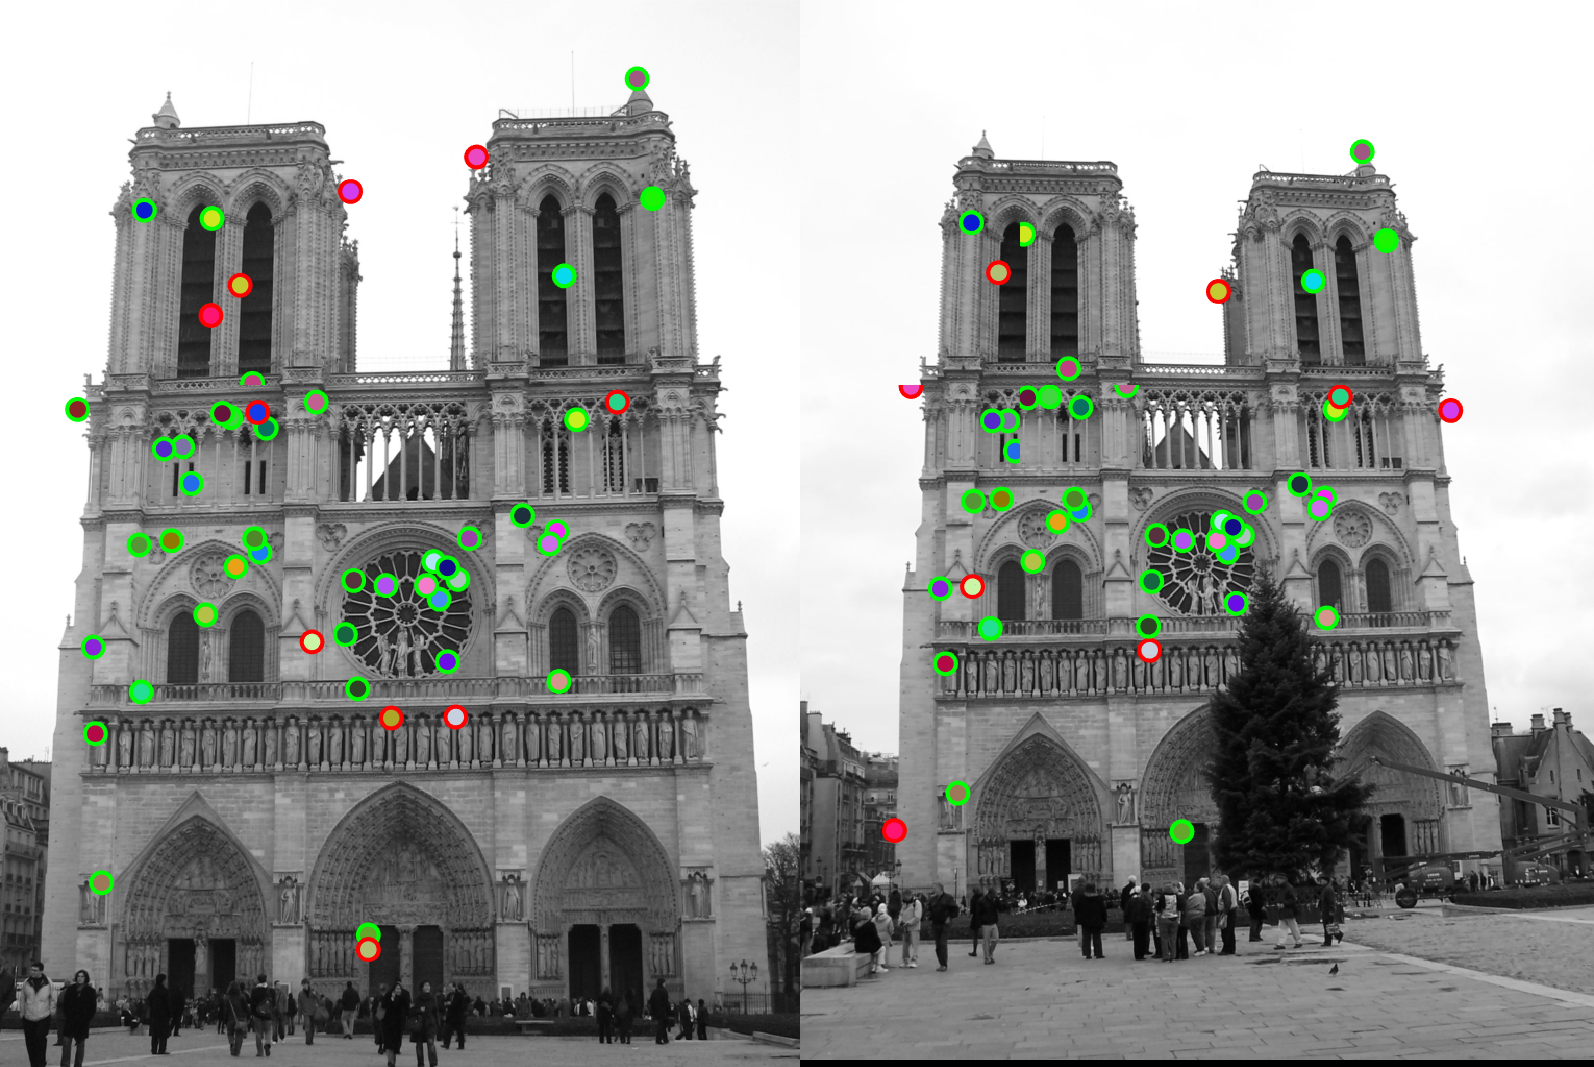
\includegraphics[width=8cm]{eval_ND.png}
    \caption{eval\_ND}
    \label{fig:result1}
\end{figure}
$1.$ Notre Dame de Paris\\
Uniqueness: Pre-merge:    51  Post-merge:  51\\
Total:      Good matches: 41  Bad matches: 10\\
Accuracy:  80.39\% (on all 51 submitted matches)\\
Accuracy:  41\% (on first 100 matches sorted by decreasing confidence)\\
\\
\begin{figure}[!h]
    \centering
    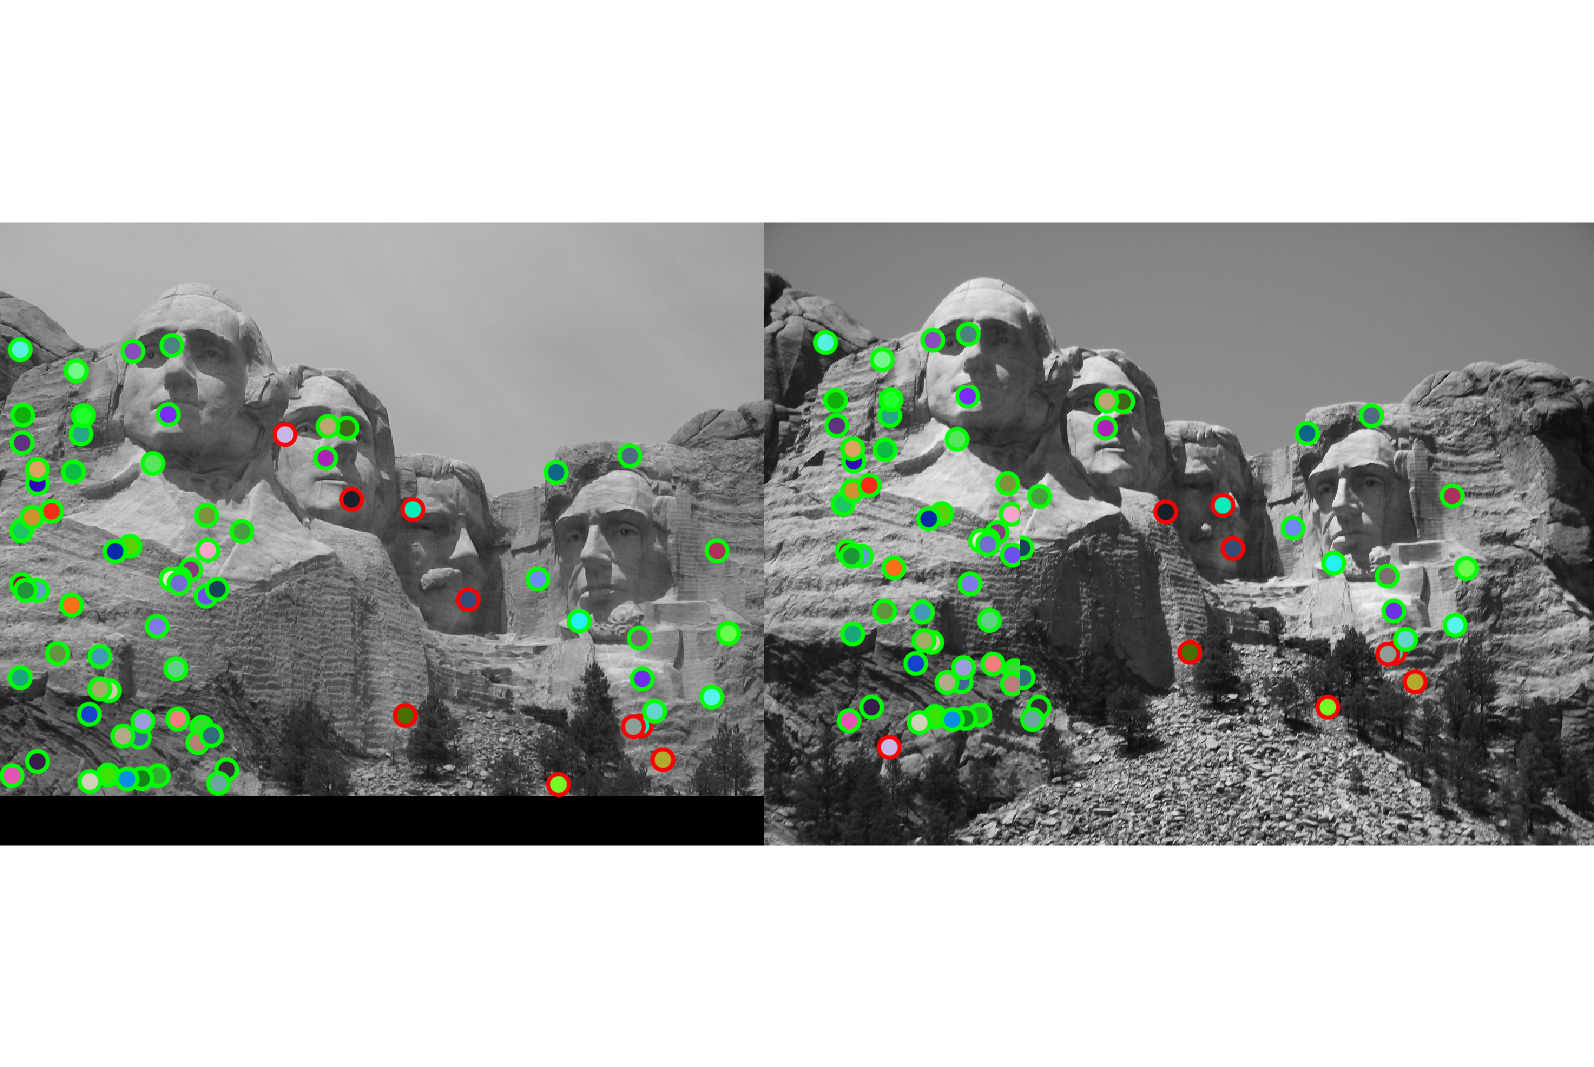
\includegraphics[width=8cm]{eval_MR.png}
    \caption{eval\_MR}
    \label{fig:result1}
\end{figure}
$2.$ Mount Rushmore\\
Uniqueness: Pre-merge:    77  Post-merge:  77\\
Total:      Good matches: 68  Bad matches: 9\\
Accuracy:  88.31\% (on all 77 submitted matches)\\
Accuracy:  68\% (on first 100 matches sorted by decreasing confidence)\\
\\
\begin{figure}[!h]
    \centering
    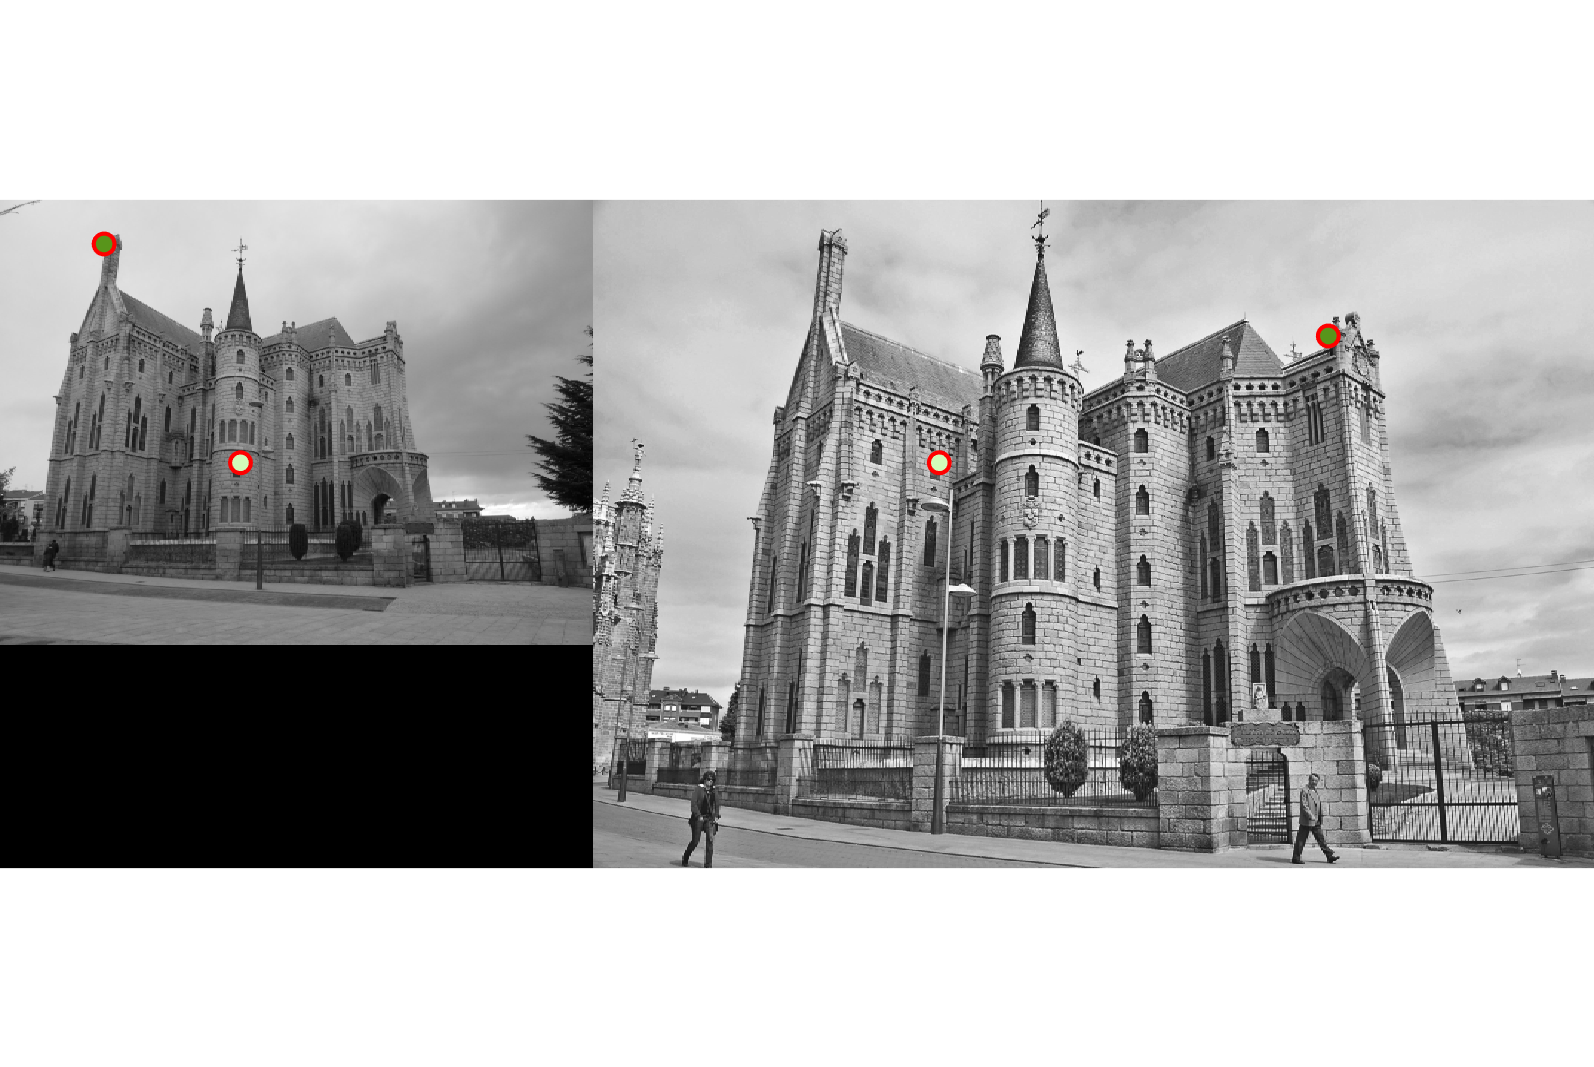
\includegraphics[width=8cm]{eval_EG.png}
    \caption{eval\_EG}
    \label{fig:result1}
\end{figure}
$3.$ Gaudi's Episcopal Palace\\
Uniqueness: Pre-merge:    2  Post-merge:  2\\
Total:      Good matches: 0  Bad matches: 2\\
Accuracy:  0\% (on all 2 submitted matches)\\
Accuracy:  0\% (on first 100 matches sorted by decreasing confidence)\\
\\
\end{document}